\documentclass[a4paper]{article}
\usepackage[utf8]{inputenc}
\usepackage{amsmath}
\usepackage[nodayofweek]{datetime}

\usepackage{tikz}

% Set size of text area with total parameter
\usepackage[a4paper, total={135mm, 255mm}]{geometry}

\title{Quarter Circles in a Semi Circle}
\author{Dyson}
\date{\today}

\begin{document}

\maketitle

% Set paragraph spacing here to avoid messing with title
\setlength{\parindent}{0em}
\setlength{\parskip}{1em}

This question wants the fraction of the area of two quarter circles divided by the area of the semi circle that bounds them.

\hspace{\fill}
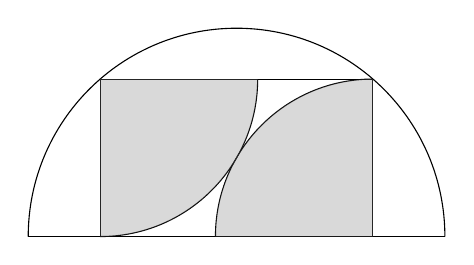
\begin{tikzpicture}
% I need to mention that this whole diagram is scaled up by 2, just to make it bigger on the page
\draw ({-sqrt(7)},0) -- ({sqrt(7)},0);
% The semi circle
\draw ({sqrt(7)},0) arc[start angle=0, end angle=180, radius={sqrt(7)}];
% The rectangluar bounding box
\draw ({-sqrt(3)},0) -- ({-sqrt(3)},2) -- ({sqrt(3)},2) -- ({sqrt(3)},0);
% The quarter circles
\draw ({sqrt(3)},2) arc[start angle=90, end angle=180, radius=2];
\draw ({-sqrt(3)},0) arc[start angle=-90, end angle=0, radius=2];
% Shade them in as well
\fill[gray,opacity=0.3] ({-sqrt(3)},2) -- ({-sqrt(3)},0) arc[start angle=270, end angle=360, radius=2];
\fill[gray,opacity=0.3] ({sqrt(3)},0) -- ({sqrt(3)},2) arc[start angle=90, end angle=180, radius=2];
\end{tikzpicture}
\hspace{\fill}

We can begin by defining the radius of the quarter circles to be 1. We can also call the remaining length along the bottom of the rectangle $x$.

\hspace{\fill}
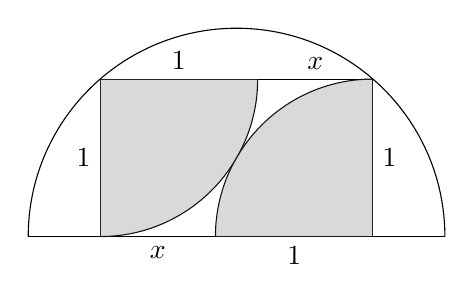
\begin{tikzpicture}
\draw ({-sqrt(7)},0) -- ({sqrt(7)},0);
\draw ({sqrt(7)},0) arc[start angle=0, end angle=180, radius={sqrt(7)}];
\draw ({-sqrt(3)},0) -- ({-sqrt(3)},2) -- ({sqrt(3)},2) -- ({sqrt(3)},0);
\draw ({sqrt(3)},2) arc[start angle=90, end angle=180, radius=2];
\draw ({-sqrt(3)},0) arc[start angle=-90, end angle=0, radius=2];
\fill[gray,opacity=0.3] ({-sqrt(3)},2) -- ({-sqrt(3)},0) arc[start angle=270, end angle=360, radius=2];
\fill[gray,opacity=0.3] ({sqrt(3)},0) -- ({sqrt(3)},2) arc[start angle=90, end angle=180, radius=2];
% The new labels
\coordinate[label=0:$1$] (1) at ({sqrt(3)},1);
\coordinate[label=270:$1$] (1) at ({sqrt(3)-1},0);
\coordinate[label=180:$1$] (1) at ({-sqrt(3)},1);
\coordinate[label=90:$1$] (1) at ({1-sqrt(3)},2);
\coordinate[label=90:$x$] (x) at (1,2);
\coordinate[label=270:$x$] (x) at (-1,0);
\end{tikzpicture}
\hspace{\fill}

Now, to find $x$, we can define the diagonal length $\ell$ in two ways. I'll remove the shading to make things easier to see.

\hspace{\fill}
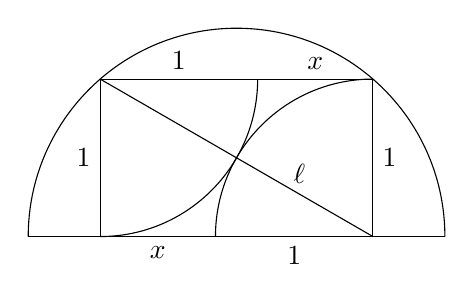
\begin{tikzpicture}
\draw ({-sqrt(7)},0) -- ({sqrt(7)},0);
\draw ({sqrt(7)},0) arc[start angle=0, end angle=180, radius={sqrt(7)}];
\draw ({-sqrt(3)},0) -- ({-sqrt(3)},2) -- ({sqrt(3)},2) -- ({sqrt(3)},0);
\draw ({sqrt(3)},2) arc[start angle=90, end angle=180, radius=2];
\draw ({-sqrt(3)},0) arc[start angle=-90, end angle=0, radius=2];
\coordinate[label=0:$1$] (1) at ({sqrt(3)},1);
\coordinate[label=270:$1$] (1) at ({sqrt(3)-1},0);
\coordinate[label=180:$1$] (1) at ({-sqrt(3)},1);
\coordinate[label=90:$1$] (1) at ({1-sqrt(3)},2);
\coordinate[label=90:$x$] (x) at (1,2);
\coordinate[label=270:$x$] (x) at (-1,0);
% ell
\draw ({-sqrt(3)},2) -- ({sqrt(3)},0);
\coordinate[label=0:$\ell$] (ell) at (0.6,0.8);
\end{tikzpicture}
\hspace{\fill}

Because the two quarter circles are centred at opposite corners of the rectangle, the diagonal line $\ell$ must pass through their kissing point. This means that $\ell$ is the sum of the quarter circles' radii, so $\ell = 2$.

Alternatively, we can use Pythagoras to get $\ell = \sqrt{1^2 + (x + 1)^2} = \sqrt{x^2 + 2x + 2}$. Therefore, we can say that $2 = \sqrt{x^2 + 2x + 2}$. We can then solve for $x$.
\begin{gather*}
4 = x^2 + 2x + 2\\
x^2 + 2x - 2 = 0\\
x = -1 \pm \sqrt{3}
\end{gather*}
$x$ is a distance, so it must be positive, which means that $x = -1 + \sqrt{3}$.

\newpage

Before computing any areas to get our answer, we need to be able to find the area of the semi circle. To do this, we need the radius. To find the radius, we need the midpoint, which is the projection of the kissing point onto the horizontal line.

\hspace{\fill}
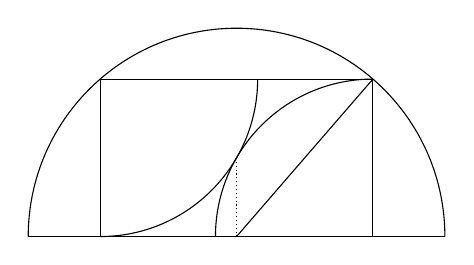
\begin{tikzpicture}
\draw ({-sqrt(7)},0) -- ({sqrt(7)},0);
\draw ({sqrt(7)},0) arc[start angle=0, end angle=180, radius={sqrt(7)}];
\draw ({-sqrt(3)},0) -- ({-sqrt(3)},2) -- ({sqrt(3)},2) -- ({sqrt(3)},0);
\draw ({sqrt(3)},2) arc[start angle=90, end angle=180, radius=2];
\draw ({-sqrt(3)},0) arc[start angle=-90, end angle=0, radius=2];
\draw (0,0) -- ({sqrt(3)},2);
\draw[densely dotted] (0,0) -- (0,1);
\end{tikzpicture}
\hspace{\fill}

It's quite hard to find the midpoint. However, it's quite easy to simply reflect the circle and bounding box in the horizontal axis and continue this line to be a diameter.

\hspace{\fill}
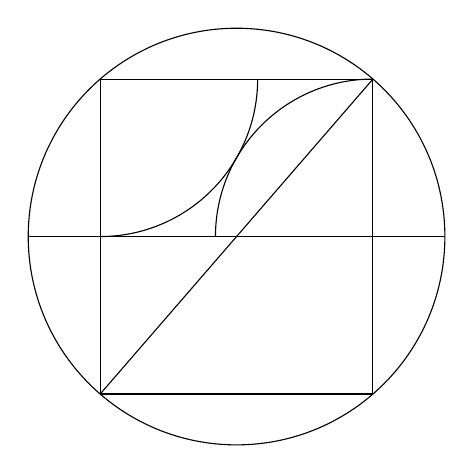
\begin{tikzpicture}
\draw ({-sqrt(7)},0) -- ({sqrt(7)},0);
\draw ({sqrt(7)},0) arc[start angle=0, end angle=360, radius={sqrt(7)}];
\draw ({-sqrt(3)},-2) -- ({-sqrt(3)},2) -- ({sqrt(3)},2) -- ({sqrt(3)},-2) -- cycle;
\draw ({sqrt(3)},2) arc[start angle=90, end angle=180, radius=2];
\draw ({-sqrt(3)},0) arc[start angle=-90, end angle=0, radius=2];
\draw ({-sqrt(3)},-2) -- ({sqrt(3)},2);
\end{tikzpicture}
\hspace{\fill}

We can then add our lengths back on to the diagram and use Pythagoras to find this diameter.

\hspace{\fill}
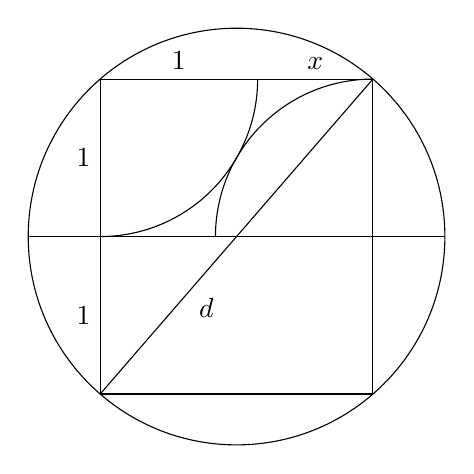
\begin{tikzpicture}
\draw ({-sqrt(7)},0) -- ({sqrt(7)},0);
\draw ({sqrt(7)},0) arc[start angle=0, end angle=360, radius={sqrt(7)}];
\draw ({-sqrt(3)},-2) -- ({-sqrt(3)},2) -- ({sqrt(3)},2) -- ({sqrt(3)},-2) -- cycle;
\draw ({sqrt(3)},2) arc[start angle=90, end angle=180, radius=2];
\draw ({-sqrt(3)},0) arc[start angle=-90, end angle=0, radius=2];
\draw ({-sqrt(3)},-2) -- ({sqrt(3)},2);
\coordinate[label=180:$1$] (1) at ({-sqrt(3)},1);
\coordinate[label=90:$1$] (1) at ({1-sqrt(3)},2);
\coordinate[label=90:$x$] (x) at (1,2);
\coordinate[label=180:$1$] (1) at ({-sqrt(3)},-1);
\coordinate[label=0:$d$] (d) at (-0.6,-0.9);
\end{tikzpicture}
\hspace{\fill}

We can now see that the diameter $d$ is simply $\sqrt{2^2 + (x + 1)^2}$. Since $x = -1 + \sqrt{3}$, we know that $x + 1 = \sqrt{3}$, so $d = \sqrt{4 + 3} = \sqrt{7}$. That means that the radius of the big circle is $\frac{\sqrt{7}}{2}$.

Now we can compute the fraction of area that we want. The area of the two quarter circles is $2 \times \frac{\pi}{4} \times 1^2 = \frac{\pi}{2}$. The area of the original semi circle is $\frac{\pi}{2} \times \left(\frac{\sqrt{7}}{2}\right)^2 = \frac{7 \pi}{8}$.

We divide these areas and we get $\displaystyle \frac{\pi}{2} \div \frac{7 \pi}{8} = \frac{4}{7} \approx 57.1\%$, which is our final answer.

\end{document}
